% ============================================================================
% 20_results.tex  --  Methods & results  (~2 pages)
% Figures: block1.py figs 4, 5, 6, 9, 10 (this part's block), regenerated fresh:
%   python src/block1.py --plots 4            (L=30)
%   python src/block1.py --plots 5 --L 20
%   python src/block1.py --plots 6 9 --L 100
%   python src/block1.py --plots 10 --L 20
% ============================================================================

\section{Methods and results}
\label{sec:results}

All results are exact diagonalisations of the BdG matrix \eqref{eq:bdg} at
$t = \Delta = 1$ unless stated otherwise, obtained with the symmetric
eigensolver \texttt{numpy.linalg.eigvalsh} in double precision. Quasiparticle
energies are taken as $\mathrm{sort}(|E|)$ keeping one entry per $\pm E$ pair,
rather than by filtering on the sign of $E$.

\subsection{OBC spectrum and the two mid-gap levels}
\label{sec:obc}
Figure~\ref{fig:spectrum} sweeps $\mu$ through both critical points at
$L = 30$. A near-zero branch spans the whole topological window; beyond
$|\mu| = 2t$ no sub-gap state remains. At $\mu = -t$ it sits at $E_0 = 1.397 \times 10^{-9}$, matching
$2t(1-\tfrac14)(\tfrac12)^{30}$ from Eq.~\eqref{eq:splitting} to six
significant figures; at $\mu = 0$ it is $2.5 \times 10^{-16}$, zero to double
precision. The branch \emph{is} the hybridised Majorana pair; the rounded
merger at $|\mu| = 2t$ is the finite-size shadow of the bulk transition (see
[Schewtschik, Part~1]), exact closing being forbidden at finite $L$ by lesson
(iii) of Sec.~\ref{sec:quantrule}. Figure~\ref{fig:snapshot} resolves this
state by state: the $L=20$ spectrum is gapped at $\mu = -3t$ but carries two
near-zero eigenvalues inside the gap at $\mu = -t$ --- not two excitations but
the $\pm E_0$ pair of a \emph{single} level, the non-local fermion built from
the two edge Majoranas.

\begin{figure}[tb]
  \centering
  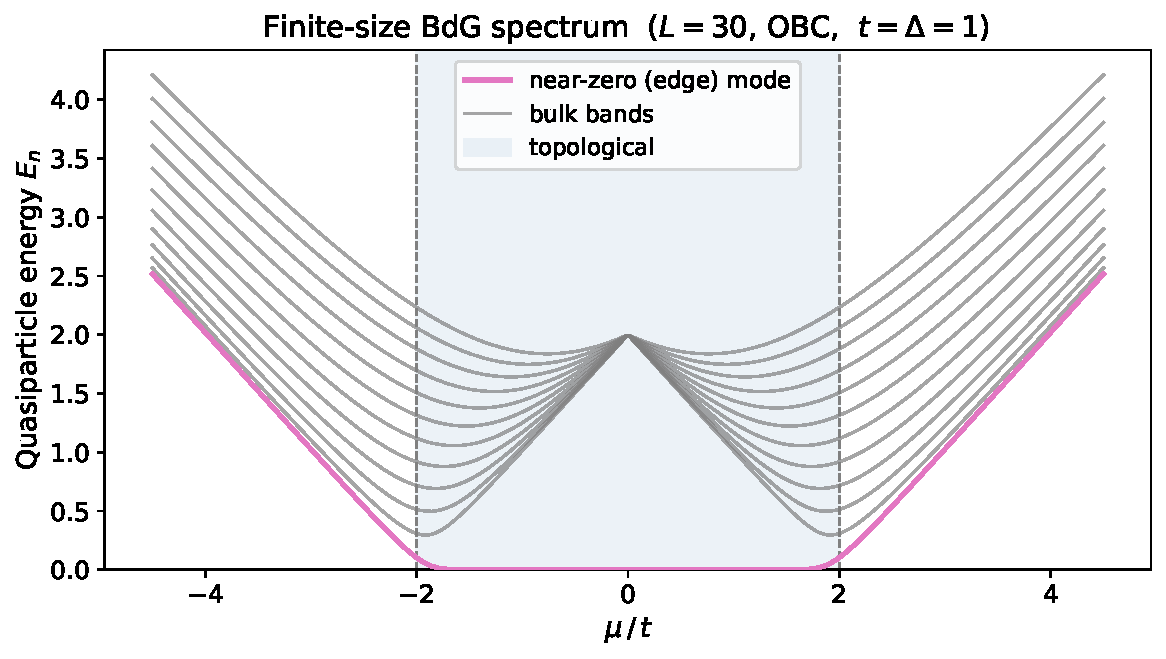
\includegraphics[width=0.60\linewidth]{figs/block1_04_finite_size_spectrum.pdf}
  \caption{Lowest twelve quasiparticle levels of the $L=30$ open chain vs
  $\mu$: the near-zero edge branch spans the topological window and merges
  into the bulk continuum at $|\mu| = 2t$.}
  \label{fig:spectrum}
\end{figure}

\begin{figure}[tb]
  \centering
  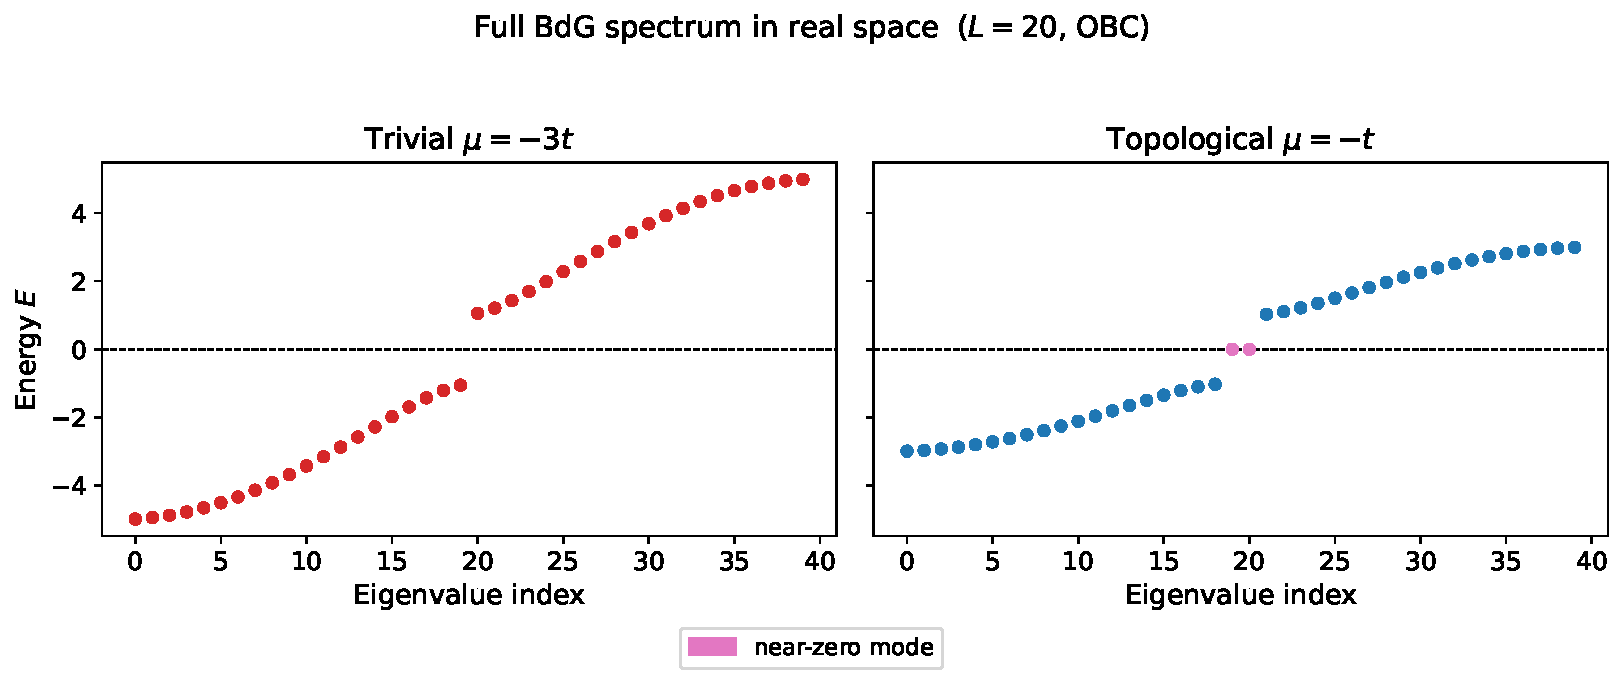
\includegraphics[width=0.72\linewidth]{figs/block1_05_realspace_snapshot.pdf}
  \caption{Full BdG spectrum of the $L=20$ open chain: trivial phase (left, no
  sub-gap states) versus topological phase (right, a single $\pm E_0$ near-zero
  pair isolated inside the gap).}
  \label{fig:snapshot}
\end{figure}

\subsection{Exponential protection: $E_0$ versus $L$}
\label{sec:scaling}
Figure~\ref{fig:splitting} shows $E_0(L)$ for $\mu/t = -0.5,-1,-1.5$ against
Eq.~\eqref{eq:splitting} (dashed). The data are straight on a semilog scale
with fitted slopes reproducing $\ln|\lambda|$, and the ratios $E_0/|\lambda|^L$
reproduce the prefactor $2t(1-\lambda^2)$, ruling out the bare estimate
$2t|\lambda|^L$ (Table~\ref{tab:fits}). The slope measures the coherence
length, $\xi = 1/|\mathrm{slope}|$: $0.7$ sites at $\mu = -0.5t$ but $3.4$ at
$\mu = -1.5t$, so protection weakens toward the phase boundary. Where the data
leave the theory lines the splitting has fallen below machine precision (at
$\mu = -0.5t$, $L = 40$ it should be $1.55 \times 10^{-24}$) and the measured
values saturate in the shaded band.

\begin{figure}[tb]
  \centering
  \begin{minipage}[t]{0.49\linewidth}
    \centering
    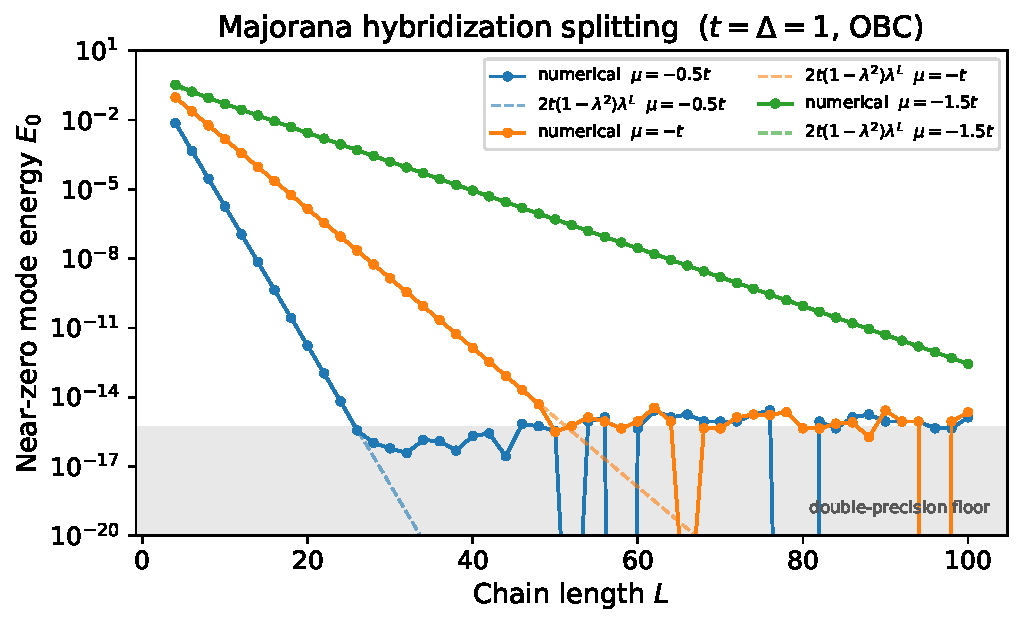
\includegraphics[width=\linewidth]{figs/block1_06_majorana_splitting.pdf}
    \caption{$E_0$ vs $L$ with Eq.~\eqref{eq:splitting} dashed: slope
    $-1/\xi$, saturating in the shaded precision band.}
    \label{fig:splitting}
  \end{minipage}\hfill
  \begin{minipage}[t]{0.49\linewidth}
    \centering
    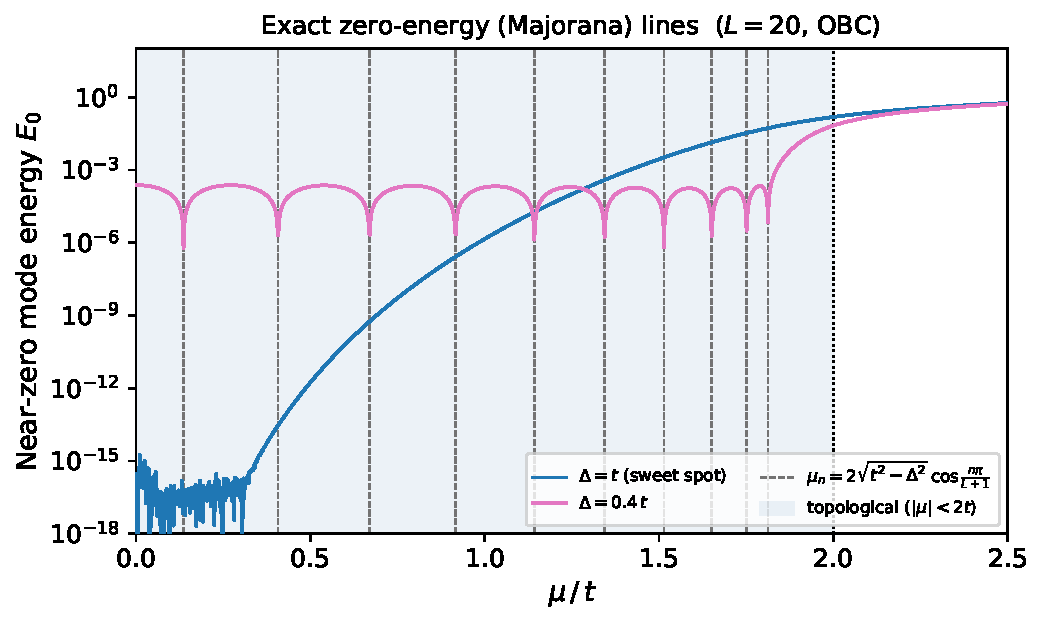
\includegraphics[width=\linewidth]{figs/block1_10_majorana_lines.pdf}
    \caption{$E_0(\mu)$ at $L = 20$: smooth at $\Delta = t$; oscillating at
    $\Delta = 0.4t$ with exact zeros on the lines $\mu_n$ of
    Eq.~\eqref{eq:majoranaline} (dashed).}
    \label{fig:majoranalines}
  \end{minipage}
\end{figure}

\begin{table}[tb]
  \centering\small
  \caption{Fits to Fig.~\ref{fig:splitting}: slopes of $\ln E_0$ vs $L$ over the
  even-$L$ grid $6,8,\dots,24$; ratios at $L = 20,40,100$ for
  $\mu/t = -0.5,-1,-1.5$ respectively (beyond those $L$ the splitting has sunk
  below machine precision and the ratio is meaningless).}
  \label{tab:fits}
  \begin{tabular}{cccccc}
    \toprule
    $\mu/t$ & fitted slope & $\ln|\lambda|$ & $E_0/|\lambda|^{L}$ &
    $2t(1-\lambda^2)$ & $\xi = 1/|\mathrm{slope}|$ \\
    \midrule
    $-0.5$ & $-1.3866$ & $-1.3863$ & $1.8748$ & $1.875$ & $0.72$ \\
    $-1.0$ & $-0.6932$ & $-0.6931$ & $1.5000$ & $1.500$ & $1.44$ \\
    $-1.5$ & $-0.2907$ & $-0.2877$ & $0.8735$ & $0.875$ & $3.44$ \\
    \bottomrule
  \end{tabular}
\end{table}

\subsection{Away from the sweet spot: Majorana lines and parity switches}
\label{sec:oscillations}
Figure~\ref{fig:majoranalines} tests Eq.~\eqref{eq:majoranaline} on one
$L = 20$ chain at two pairings. At $\Delta = t$ the splitting is a smooth
valley whose only exact zero is $\mu = 0$, where all Majorana lines coalesce.
At $\Delta = 0.4t$ it instead oscillates beneath its envelope and dips to an
exact zero at each of the ten predicted $\mu_n > 0$ (dashed), with no fit
parameter.
Diagonalisation at $\mu = \mu_n$ gives $E_0$ between $3\times10^{-18}$ and
$3\times10^{-16}$, zero to double precision, against
$E_0 \approx 2 \times 10^{-4}$ midway between lines --- twelve orders of
magnitude apart. Each $\mu_n$ is a level crossing at which the ground-state
fermion parity switches. Since a real wire is never fine-tuned to
$t = \Delta$, this oscillatory splitting --- the lattice cousin of the
Majorana oscillations of semiconductor nanowires~\cite{dassarma2012} --- is
the generic finite-size fingerprint, and Fig.~\ref{fig:splitting} its cleanest
special case.

\subsection{The sign-filter artefact}
\label{sec:artefact}
Extracting the ``positive spectrum'' naively as \texttt{evals[evals >= 0]}
produces dense spikes over most of the topological window at large $L$
(Fig.~\ref{fig:artefact}, left), while $|E|$ on the \emph{same} eigenvalues is
smooth (right). The spikes are a floating-point artefact, not
physics~\cite{goldberg1991}: the near-zero eigenvalue drops below machine
precision once
\begin{equation}
  E_0 < \varepsilon_{\mathrm{mach}}
  \quad\Longleftrightarrow\quad
  |\mu| \lesssim 2t\,\varepsilon_{\mathrm{mach}}^{1/L},
  \label{eq:threshold}
\end{equation}
i.e.\ $|\mu|_{\mathrm{thresh}} \approx 0.62$ at $L = 30$ but $\approx 1.41$ at
$L = 100$ for $\varepsilon_{\mathrm{mach}} = 5\times10^{-16}$. Inside that
window rounding can store the near-zero eigenvalue as a tiny \emph{negative}
number $\sim -10^{-16}$; the filter drops it and reports the lowest
\emph{bulk} level as ``$E_0$'' --- at $\mu = -1.38t$, $L = 100$ it returns
$0.622$ where $|E|$ gives $3.1\times10^{-15}$. Since the window \emph{widens}
with $L$, the spikes worsen for longer chains even though
Eq.~\eqref{eq:splitting} says longer chains protect the mode better --- the
counter-intuitive observation that motivated this analysis.
The lesson is to extract a symmetry-pinned quantity so that it survives
$\varepsilon$-sized violations of that symmetry --- here $|E|$ together with
pair deduplication, which is the extraction used throughout this report.

\begin{figure}[h]
  \centering
  
\includegraphics[width=0.9\linewidth]{figs/block1_09_npabs_comparison.pdf}
  \caption{Same eigenvalues, two extractions ($L=100$): the sign filter
  (left) fabricates bulk-scale spikes over the window of
  Eq.~\eqref{eq:threshold}; $|E|$ (right) resolves the near-zero mode.}
  \label{fig:artefact}
\end{figure}
